
% JuliaCon proceedings template
\documentclass{juliacon}
\setcounter{page}{1}



\usepackage{hyperref}
%\usepackage[linesnumbered,ruled,vlined]{algorithm2e}
\usepackage{graphicx}
%\usepackage[font=small,labelfont=bf]{caption}
\usepackage{subcaption}

\usepackage{tikz}
\usetikzlibrary{shapes.misc}
\tikzset{cross/.style={cross out, draw=black, thick, minimum size=2*(#1-\pgflinewidth), inner sep=0pt, outer sep=0pt},
%default radius will be 1pt. 
cross/.default={3.5pt}}
\usepackage{pgfplots}
\pgfplotsset{samples=600}
\pgfplotsset{compat=newest}
\usepackage{amsmath} 
%\usetikzlibrary{external}
%\tikzexternalize[prefix=tikz/]

\def\sinc{\mathrm{sinc}}
\def\lc{\lstinline}
\newcommand\todo[1]{\textcolor{red}{\textbf{TODO: #1}}}

\usepackage{siunitx}

\begin{document}

% **************GENERATED FILE, DO NOT EDIT**************

\title{FourierTools.jl - Working with Fourier Space}

\author[1, 2]{Felix Wechsler}
\author[1, 2, 3]{Rainer Heintzmann}
\affil[1]{Faculty of Physics and Astronomy, Friedrich-Schiller-University, Jena, Germany}
\affil[2]{Leibniz Institute of Photonic Technology, Albert-Einstein-Straße 9, 07745 Jena, Germany}
\affil[3]{Institute of Physical Chemistry and Abbe Center of Photonics, Friedrich-Schiller-University, Helmholtzweg 4, Jena, Germany}

\keywords{Julia, Fourier transform, Frequency, Signal processing}



\maketitle

\begin{abstract}
\verb|FourierTools.jl| aims at simplifying work in Fourier
space without loosing efficiency.
First, we provide several convenient wrappers to ease the usage of the common Fourier processing operations.
Second, we implement array transformations like $\sinc$ interpolation, sub pixel shifting, convolution, rotation and shearing based on Fourier transforms.
Notably, those algorithms handle the Nyquist term in case of an even sized array correctly
under the condition of minimum mean-square slope.

\end{abstract}

\section{Introduction}
The fast Fourier transform (FFT) is a popular algorithm because it can evaluate the Discrete Fourier Transform (DFT) 
\begin{equation}
    X_k = \sum_{n=0}^{N-1} x_n \exp\left(-i2 \pi \frac{kn}{N} \right)
    \label{eq:dft}
\end{equation}
and the Inverse Discrete Fourier Transform (IDFT)
\begin{equation}
    x_n = \frac1{N}\sum_{k=0}^{N-1} X_k \exp\left(i2 \pi \frac{kn}{N} \right)
    \label{eq:idft}
\end{equation}
in $\mathcal{O}(N \log N)$ operations, whereas the straightforward
evaluation takes $\mathcal{O}(N^2)$ operations.
The DFT transforms the signal to a different basis, the Fourier space which
has wide applications in signal processing.
In Julia \cite{bezanson2017julia} \verb|FFTW.jl| offers a convenient interface to
the \verb|FFTW| library \cite{FFTW05} which is among the fastest FFT libraries.
The interpretation of a signal in Fourier space is versatile and many operations can
be done using FFT operations. 
In this work, we present several operations which can be calculated quickly 
due to the good performance of FFTs.
Additionally, we also stick to a certain boundary handling in all algorithms.
All algorithms and examples are implemented using the Julia package \verb|FourierTools.jl|\footnote{The full source is available on GitHub: \url{https://github.com/bionanoimaging/FourierTools.jl/}}.

\section{Mathematical Background}
    Essential for the understanding of the algorithms presented here, is the Discrete Fourier series (DFS).
    Qualitatively, the DFS is a weighted sum of complex $\cos$ and $\sin$ terms.
    In our notation, the DFS of a signal defined in $[0, L)$ is defined as
    \begin{align}
        x_n &= \frac1{N}\sum_{k=0}^{N-1} X_k \cdot \exp\left(i2\pi \frac{k}{N} n \right) \\
        &= \frac1{N}\sum_{k=0}^{N-1} X_k \cdot \left[ \cos\left(i2\pi \frac{k}{N} n \right) + i \cdot  \sin\left(i2\pi \frac{k}{N} n \right) \right]\label{eq:DFS2}\\
        &=\frac1{N}\sum_{k=-\lfloor N/2\rfloor}^{\lceil N/2 -1 \rceil} X_k \cdot \left[ \cos\left(i2\pi \frac{k}{N} n \right) + i \cdot  \sin\left(i2\pi \frac{k}{N} n \right) \right]\label{eq:DFS}
    \end{align}
    which is the same as the IDFT definition in \autoref{eq:idft}.
    The brackets $\lfloor \cdot \rfloor$, $\lceil \cdot \rceil$ denote the floor, next lower integer number and the ceil, next upper inter number respectively. In fact, the coefficients $X_k$ are obtained with the DFT.
    \autoref{eq:DFS} can be derived from the $2\pi$ periodicity of $\sin$ and $\cos$.
    An inherent assumption of the DFS is that the signal $x_n$ is circular repeating.
    So whenever a DFT/IDFT is calculated, this property is included.
    The coefficients $X_K$ describe the strength of an individual complex
    exponential basis function.
    In general, coefficients $X_k$ are complex valued but for real input data $x_n$ it follows that
    \begin{equation}
        X_{N-k} = X_k^*.
        \label{eq:symmetry}
    \end{equation}
    This property is usually called \textit{Hermitian}.
%    \begin{figure}
%        \centering
%        \begin{tikzpicture}
%            \def\myradius{1.6}
 %           \def\mydiff{0.3}
 %           \draw[->] (-\myradius - \mydiff, 0) -- (+\myradius + \mydiff,0) node[right] {$\mathrm{Re}$};
%            \draw[->] (0, -\myradius - \mydiff) -- (0, +\myradius + \mydiff) node[right] {$\mathrm{Im}$};
%            \draw (0,0) circle(\myradius);
 %           \foreach \i in {0, 1, ..., 6}{
%                \pgfmathsetmacro{\anglee}{360/7 * \i}
%            }
%        \end{tikzpicture}
%        \caption{Caption}
%        \label{fig:dft}
%    \end{figure}

    As seen from \autoref{eq:DFS}, the maximum frequency of a signal described with the DFS is $-\lfloor N/2 \rfloor / L$ (the border of the summation interval of $k = -\lfloor N/2 \rfloor$)\footnote{You might wonder why the maximum frequency in \autoref{eq:DFS2} would be at $k=N-1$. However, this frequency is not Nyquist sampled\footnote{According to the Whittaker–Nyquist–Shannon 
        theorem \cite{whittaker_e_t_1915_1428702}, \cite{Shannon1949}.} and leads to aliasing which results that those frequencies appear at lower frequencies.}. 
    For a signal (over the range $[0, L)$) with 7 elements, the frequencies in the Fourier series would be
    \begin{equation}
        f_{\{k\}} = \left[-\frac{3}{7 L} , -\frac{2}{7 L},  -\frac{1}{7L}, \frac{0}{7L}, \frac{1}{7L}, \frac{2}{7L}, \frac{3}{7L} \right]
        \label{eq:7elems}
    \end{equation}
    and for one with 6 elements
    \begin{equation}
       f_{\{k\}} = \left[-\frac{4}{8 L} ,-\frac{3}{8 L} ,-\frac{2}{8 L} ,-\frac{1}{8 L} ,\frac{0}{8 L} ,\frac{1}{8 L} ,\frac{2}{8 L} ,\frac{3}{8 L} \right].
       \label{eq:6elems}
    \end{equation}
    The highest frequency $-\frac{4}{8 L}$ in \autoref{eq:6elems} does not fulfill Nyquist sampling and thus 
    cannot be interpreted uniquely. As drawn in \autoref{fig:nyquist_sample}, comparing the solid green, red and blue curves, there are infinitely many periodic functions of one and the same coarsest frequency
     (varying in phase and amplitude) exhibiting same sampled values.
    \begin{figure}
        \centering
        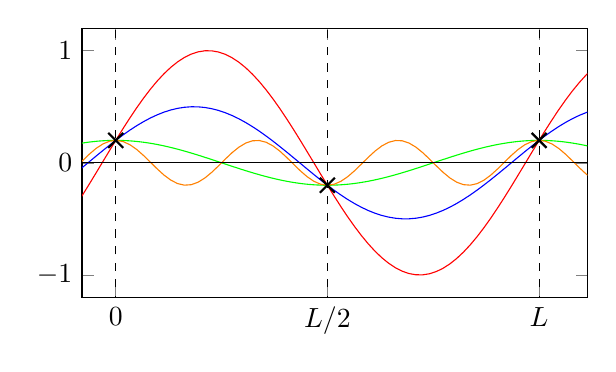
\begin{tikzpicture}
            \begin{axis}[xmin=-0.5, xmax=7, ymax=1.2, ymin=-1.2, width=8cm, height=5cm,
                xtick = {0, 3.1415, 2 * 3.1414}, xticklabels={0, $L/2$, $L$}]
                    \addplot[sharp plot, domain=-1:9, color=green, samples=400] {0.2 * cos(deg(x)};
                    \addplot[sharp plot, domain=-1:9, color=blue, samples=100] {0.5 * cos(deg(x) - 66.42};
                    \addplot[sharp plot, domain=-1:9, color=red, samples=100] {1 * cos(deg(x) - 78.46};
                    \addplot[sharp plot, domain=-1:9, color=orange, samples=100] {0.2*cos(deg( 3 *x))};
                    \draw[] (axis cs:-1, 0) -- (axis cs:8, 0);
                    \draw[dashed] (axis cs:0, -2) -- (axis cs:0, 2);
                    \draw[dashed] (axis cs:3.1415, -2) -- (axis cs:3.1415, 2);
                    \draw[dashed] (axis cs:3.1415*2, -2) -- (axis cs:3.1415*2, 2);
                    
                    
                   \draw (0,0.2) node[cross, thick] { };
                    \draw (3.1415,-0.2) node[cross, thick] { };
                     \draw (2 * 3.1415,0.2) node[cross, thick] { };

            \end{axis}
        \end{tikzpicture}
        \caption{Periodic signal of period length $2\pi$ which has been sampled with $\pi$ spacing.}
        \label{fig:nyquist_sample}
    \end{figure}
    
    Coming back to \autoref{eq:7elems} we can think about what happens if we extend the Fourier spectrum by introducing additional frequencies. 
    For example, we can symmetrically introduce higher frequencies, which we pretend to have measured but which yielded zero amplitude. That means, that we do not add new information to our measured information.
    However, calculating the IDFT we now evaluate the Fourier series on a different grid.
    By our introduction of higher frequencies with zero strength, we did not change the domain of the function but we simply evaluate the Fourier series at a denser spaced grid in real space. This evaluation changes the signal to a smother, \textit{interpolated} appearance.
    The whole procedure is called Sinc \textit{interpolation}.\\
    
    \subsection{Sinc Upsampling of Real--Valued Signals}
        Now we discuss how we apply $\sinc$ interpolation to of real--valued signals.
        Starting with an odd-sized signal is simple (see above) as we only have to pad with zeros.
        Starting with an even-sized signal is more difficult, which is demonstrated in the next parts.
        
        \subsubsection{Even $\rightarrow$ Odd}
            If we consider a real signal (with length $N=4$) $[x_0, x_1, x_2, x_3]$ we discuss how to interpolate
            this signal to a length of $N=5$ and $N=6$.
            The frequencies of the signal shall be called $[X_{-2}, X_{-1}, X_0, X_1]$.
            Interpolation to a length $N=5$, naively we would think that padding the frequencies to
            \begin{equation}
                Y_k = [X_{-2}, X_{-1}, X_0, X_1, 0]
            \end{equation}
            would be sufficient. However, because of \autoref{eq:symmetry} the resulting signal
            \begin{equation}
                y_n = \mathcal{F}^{-1}\left[X_{-2}, X_{-1}, X_0, X_1, 0\right]
            \end{equation}
            is not real anymore. In our opinion, a real interpolated signal
            should result in a real signal after interpolation.
            Therefore, we have to restore the symmetry property, resulting in a real signal.
            To achieve that, one way would be to equally split the real--valued Nyquist amplitude (the highest frequency) equally between two highest frequencies like
            \begin{equation}
                y_n = \mathcal{F}^{-1}\left[X_{-2} / 2, X_{-1}, X_0, X_1, X_{-2}/2 \right].
            \end{equation}
            This choice of interpolation warrants real values of $y_n$ and additionally, minimizes the mean-square slope\footnote{This has been derived by Steven G. Johnson: \url{https://discourse.julialang.org/t/sinc-interpolation-based-on-fft/52512/82}.
            There are also additional notes here: \url{https://math.mit.edu/~stevenj/fft-deriv.pdf}.}. Note, that since $X_{-2}$ is guaranteed to be real for real--valued signals, no complex conjugation is required in the split for one-dimensional Fourier-transformations.
        
        \subsubsection{Even $\rightarrow$ Even}
            To interpolate to $N=8$ we can then do
            \begin{equation}
                y_n = \mathcal{F}^{-1}\left[0, 0, X_{-2} / 2, X_{-1}, X_0, X_1, X_{-2}/2, 0 \right].
            \end{equation}
            The limit--frequency is split as before and all frequencies above the initial Nyquist amplitude are set to zero.
            
        \subsubsection{Odd $\rightarrow$ Odd}
            The odd case is straightforward, starting with the frequencies
            \begin{equation}
                X_k = [X_{-1}, X_0, X_1]
            \end{equation}
            going to a larger odd or even array by zero--padding, always fulfills the real property.
            \begin{equation}
                y_n = \mathcal{F}^{-1}[0, X_{-1}, X_0, X_1, 0]
            \end{equation}
            
        \subsubsection{Odd $\rightarrow$ Even}
            Also for the even case, the all new frequencies are set to zero including the new Nyquist frequency.
            \begin{equation}
                y_n = \mathcal{F}^{-1}\left[0, X_{-1}, X_0, X_1\right].
            \end{equation}
    
    
    \subsection{Sinc Downsampling}
        Instead of upsampling the signal, we can also remove higher frequency content.
        The result is a signal which in principle is free of aliasing, as opposed to for example binning of adjacent pixels, which would result in aliasing.
        
        \subsubsection{Even $\rightarrow$ Odd}
            We can simply remove the Nyquist amplitude.
            Starting from $[X_{-2}, X_{-1}, X_0, X_1]$ downsampling to $N=3$ is 
            \begin{equation}
                Y_k = [X_{-1}, X_0, X_1].
            \end{equation}
        \subsubsection{Even $\rightarrow$ Even}
            However, going to $N=2$ we have to accumulate the two highest frequencies into the one remaining Nyquist amplitude: 
            \begin{equation}
                Y_k = [X_{-1} + X_{1}, X_0].
            \end{equation}
            The qualitative meaning is, that since we only have a single negative Nyquist amplitude, this frequency is aliased (positive counter--part is missing) and this negative Nyquist amplitude stores the sum of both entries. Note that also here, no complex conjugation is applied to yield a real-valued Nyquist frequency, forcing the resulting signal $y_n$ to be real (see symmetry property \autoref{eq:symmetry}), .
            
        \subsubsection{Odd $\rightarrow$ Odd}
            We can downsample 
            \begin{equation}
                Y_k = [X_{-2}, X_{-1}, X_0, X_1, X_2]
            \end{equation}
            to an odd--sized array in a straight--forward way by dropping the surplus frequencies:
            \begin{equation}
                Y_k = [X_{-1}, X_0, X_1].
            \end{equation}
            
       \subsubsection{Odd $\rightarrow$ Even}
           Going to an even sized signal is again achieved by accumulating the Nyquist amplitude entry:
            \begin{equation}
                Y_k = [X_{-1} + X_1, X_0].
            \end{equation}
        In summary, for upsampling only the source even--sized arrays and for downsampling only the destination even-sized arrays require a special treatment.
        It is worth stressing that the Nyquist-frequency data in even-sized signals has no unique interpretation neither for real nor for complex valued data many combinations of underlying amplitude and phase yield the same sampled signal. Therefore, first downsampling to an even-sized array followed by upsampling will in general be modifying this downsampled Nyquist--frequency, which can only be avoided if additional assumptions can be made. Ideally, the user should avoid data being present at this even-sized Nyquist frequency, to avoid ambiguities.
        Finally, real--valued signals should be interpolated by exploiting real--to--complex Fourier transform algorithms, as this comes with increased speed and reduced memory consumption. Yet the considerations presented above apply in an analogous way.
    \subsection{Sinc Interpolation in $N$ Dimensions}
        The multidimensional signal handling is in principle similar as for 
        a 1D dataset. However, the Nyquist amplitude is not a single entry anymore but rather a $(N-1)$--dimensional hyperplane.
        \subsubsection{Odd Case}
            Assuming the real dataset $x_{i,j}$, we obtain its DFT as
            \begin{equation}
                X_{k, m} = \begin{bmatrix}
                   X_{-1, -1} &  X_{-1, 0} \\ 
                   X_{0,-1} & X_  {0, 0} \\
                \end{bmatrix}
            \end{equation}
            The interpolation to a $3\times 3$ array  $y_{\{i, j\}}$, needs the following form
            \begin{equation}
                y_{i, j} = \mathcal{F}^{-1}\begin{bmatrix}
                   X_{-1, -1}/2 &  X_{-1, 0}/2  & 0\\ 
                   X_{0,-1}/2   & X_{0, 0}      &  X_{0,-1}^*/2\\
                    0           &  X_{-1, 0}^*/2 &  X_{-1, -1}^*/2\\
                \end{bmatrix}
            \end{equation}
            Note, in $N>1$ dimensions we need to adhere to the \textit{Hermitian} property for the
            resulting signal to be real. 
            For a 1D signal the Nyquist term is real and hence complex conjugation was not necessary but in $N>1$ complex conjugation seems to be required.\\
            However, due to the separability of the DFT, we can  interpolate each dimension separately.
            This allows us to treat any N dimensional signal as a collection of 1D signals, treating each dimension individually but simultaneously for all such 1D signals.
            The first interpolation along the first dimension would be
            \begin{equation}
                y^{1}_{i, j} = \mathcal{F}_{m}^{-1}\begin{bmatrix}
                   X^1_{-1, -1}/2 &  X^1_{-1, 0}/2 \\ 
                   X^1_{0,-1} & X^1_{0, 0} \\
                   X^1_{-1,-1}/2 & X^1_{-1, 0}/2 \\
                \end{bmatrix}
            \end{equation}
            and with the new coefficients $\mathcal{F} \left[y^{1}_{\{i, j\}} \right] =Y^{1}_{k, m} $  
            If we interpolate this intermediate result along the second dimension we obtain
            \begin{equation}
                y^{1,2}_{k, m} = \mathcal{F}_{k}^{-1}\begin{bmatrix}
                   Y^1_{-1, -1} /2 &  Y^1_{-1, 0} & Y^1_{-1, -1} / 2\\ 
                   Y^1_{0,-1} /2& Y^1_{0, 0} & Y^1_{0, -1} / 2\\
                   Y^1_{-1,-1}/2 & Y^1_{-1, 0}& Y^1_{-1, -1} / 2\\ 
                \end{bmatrix}.
            \end{equation}
            The advantage of this method is the easier boundary handling since we only 
            need to divide the $N-1$ dimensional slice and do not have to care about maintaining the 
            Hermitian property (which is more difficult to program).
            In the even case, the Nyquist amplitude gets aliased and hence we would have
            to add the $(N-1)$ dimensional slices together in a flipped way.
            But again, doing that sequentially is simpler because there is no need to flip the data. 
            
        \subsubsection{Downsampling}
            As described in the 1D case, for downsampling to an even-sized array we have to 
            add the two highest frequencies to yield one new Nyquist amplitude. For $N$ dimensions this 
            procedure works sequentially over the dimensions as described in the upsampling routine.
            
            
    \subsection{Convolution Theorem}
        The convolution theorem states that a convolution can be expressed as
        a point wise multiplication and three Fourier transforms,
        \begin{equation}
            u * v = \mathcal{F}^{-1}\left[\mathcal F[u] \cdot \mathcal{F}[v]\right]
        \end{equation}
        where $*$ is the convolution and $\cdot$ the point wise multiplication.
        This property can be proved with the usage of the DFT definition (see \autoref{eq:dft}).
        A FFT based convolution usually offers an improvement if the kernel $u$ is large.
        
    \subsection{Shift Theorem}
        The Fourier Shift theorem tells us that a shift of a signal can be calculated 
        in Fourier space the point wise multiplication of the Fourier--transformed signal by a complex-valued phase ramp.
        This is directly derived from the DFT definition.
        The full form of the Fourier shift theorem is:
        \begin{equation}
            u(\mathbf x+ \Delta \mathbf x) = \mathcal{F}^{-1}\big[\mathcal{F}[u(\mathbf x)](\mathbf k) \cdot \exp(i \mathbf k \Delta \mathbf x) \big]
            \label{eq:shifting}
        \end{equation}
        where $\Delta x$ can be an arbitrary shift not restricted to integer values.
        \subsubsection{Handling of the Nyquist Amplitude}
            As before, separate handling of the Nyquist amplitude is essential, otherwise 
            the real symmetry property might be violated leading to a complex--valued output for a real input.
            \autoref{eq:shifting} can be also interpreted as a convolution of the signal $u$
            with the kernel $\mathcal{F}^{-1}\left[\exp(i \mathbf k \Delta \mathbf x)\right]$.            
            Hence, this kernel should be purely real in real space, otherwise the
            shifting kernel does mix real and imaginary part of the signal.
            For a real signal not observing this kernel--property would introduce an imaginary part, for a purely imaginary signal it would introduce real values, and for a complex--valued signal it would mix both of them. We thus need to ensure a real--valued kernel. The complex exponential in \autoref{eq:shifting} has the required Hermitian property except for its value at the Nyquist--frequency in case of even--sized arrays. In this case we only multiply by the real part of the phase factor! Note that this yield to a positive and negative shift operation not perfectly compensating each other. Another consequence of the undefined underlying signal. This effect can be avoided and a reversible shift can be guaranteed by setting this frequency of the kernel to the real value of 1.0 but this might be less accurate on average for the shift. Note that for shifts not being exactly half-pixels, the inverse shift can be modified such that it perfectly recreates the original signal, even if the first shift used the real part of the kernel at Nyquist--frequency, if the user knows that the operation is an inverse shift: We simply need to replace the real part with one over the real part. 
            
        \subsection{Shifting in $N$ Dimensions}
            As for multidimensional $\sinc$ interpolation, we similarly can process the shifting in multiple dimensions sequentially.
            
    \subsection{Array Shearing}
        Since we can shift data by an arbitrary amount via the shift theorem, 
        we can apply it with varying amounts of shifts between the $(N-1)$ dimensional hyperplanes of an $N$ dimensional array. If we vary the shifts linearly with position we obtain a sheared version of the input signal.
            
    \subsection{Array Rotation}
        A very simple image rotation algorithm is the "three shear algorithm" \cite{Paeth1986:15}.
        Its essence is that a rotation in two dimensions can be implemented by shearing an image first horizontally, then vertically and finally horizontally again.
        Mathematically, the rotation matrix (in 2D) with rotation angle $\theta$ can be separated into three shear matrices:
        \begin{equation}
            \begin{pmatrix}
                \cos(\theta) & -\sin(\theta)\\
                \sin(\theta) & \phantom{-}\cos(\theta)
            \end{pmatrix} 
            =  \begin{pmatrix}
                1 & \alpha\\
                0 & 1
            \end{pmatrix}
            \cdot
             \begin{pmatrix}
                1 & 0\\
                \beta & 1
            \end{pmatrix}
            \cdot
             \begin{pmatrix}
                1 & \alpha\\
                0 & 1
            \end{pmatrix}
        \end{equation}
        The new parameters are $\alpha=-\tan\left(\frac{\theta}{2} \right)$ and $\beta=\sin(\theta)$\footnote{See also the more detailed notes of Tobin Fricke: \url{https://www.ocf.berkeley.edu/~fricke/projects/israel/paeth/rotation_by_shearing.html}.}.
        Since shearing is a shift operation with different amounts along each line, the complete rotation
        can be fully expressed with Fourier transforms and element--wise multiplications. Note that care has to be taken to provide additional padding prior to shifting, as the Fourier--based shifts (and thus also the shears) are cyclic in nature.

    

\section{Examples}
    In this part we present the main contributions of \verb|FourierTools.jl| which
    include \lstinline{fftshift} alternatives, wrappers for \lstinline{fft}, $\mathrm{sinc}$ interpolation, convolutions and shifting, shearing and rotation.
    Our experiments additionally made use of the packages ArrayInterface.jl\cite{DifferentialEquations.jl-2017}, BenchmarkTools.jl\cite{BenchmarkTools.jl-2016} .
    
    \subsection{FFT Helpers}
        A very common pattern in signal processing is to apply various frequency filters
        which are multiplied by the signal in Fourier space. 
\begin{lstlisting}[language=Julia, caption={Typical workflow to manipulate the data in Fourier space. Note that it would be also possible to \lc{ifftshift(mask)} instead of rearranging the data twice. However, this breaks apart once one has a non-straightforward accessing scheme instead of a plain array which is multiplied.}, 
label = {lst:example_render}, 
captionpos = b,]
function fft_filter(arr, mask)
    arr_ft = fftshift(fft(arr))
    arr_ft .*= mask
    ifft(ifftshift(arr_ft))
end

function ffts_filter(arr, mask)
    arr_ft = ffts(arr) 
    arr_ft .*= mask
    iffts(arr_ft)
end
\end{lstlisting}


Our package provides \lc{ffts} and \lc{iffts} which automatically applies \lc{fftshift} and \lc{ifftshift} after respectively before calling \lc{fft}.
\lc{fftshift} and \lc{ifftshift} also copy and reshuffle the data. We instead make use of the package
\verb|ShiftedArrays.jl|\footnote{See \url{https://github.com/bionanoimaging/ShiftedArrays.jl}. Thanks
to Pietro Vertechi who supported us in implementing \lc{ShiftedArrays.fftshift} and \lc{ShiftedArrays.ifftshift}}
By keeping track of the total shifts we can avoid to copy the data in between using the \lc{fftshift} and \lc{ifftshift} but instead return the original data.

In \autoref{code:ffts} we can see the simple benchmark showing the computing time and the total
allocations needed.
\begin{lstlisting}[language=Julia, label={code:ffts}, caption={By using \lc{ffts} we can save a factor of 2 in memory}, captionpos=b]
julia> using FourierTools, BenchmarkTools, FFTW, IndexFunArrays
julia> N = (4000, 3001);
julia> arr = randn(ComplexF32, N); # 91.583 MiB
julia> mask = IndexFunArrays.rr(Float32, N) .< 50; # low pass
julia> @btime fft_filter($arr, $mask); # using fftshift
  604.883 ms (78 allocations: 366.34 MiB)
julia> @btime ffts_filter($arr, $mask); # using a fftshift_view
  596.754 ms (54 allocations: 183.17 MiB)
\end{lstlisting}

Additionally, to \lc{ffts}, inspired by DipImage\footnote{\url{https://diplib.org/}}, we also provide \lc{ft} which does both a shifting before and after calling \lc{fft}.
The schematic behavior of all different methods is drawn in \autoref{fig:freq_pos}.
    \begin{figure}[h]
        \centering
        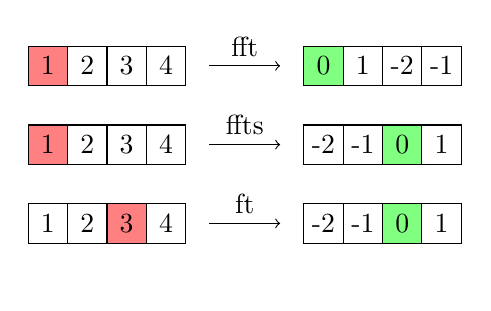
\begin{tikzpicture}
            \begin{scope}[shift={(0,00)}]
                \draw[->] (2.3, 0.25) -- (3.2, 0.25) node[midway, above] {\lc{fft}};
                \draw[fill=red!50!white] (0, 0) rectangle (0.5, 0.5);
                \draw[fill=green!50!white] (3.5, 0) rectangle (4.0, 0.5);
                \foreach \i/\j/\k in {0/0/1,1/1/2,2/-2/3,3/-1/4}{
                    \draw (\i/2, 0) rectangle (\i/2+1/2, 1/2) node[midway] {\k};
                    \draw (3.5+\i/2, 0) rectangle (3.5+\i/2+1/2, 1/2)node[midway] {\j};
                }

            \end{scope}
            \begin{scope}[shift={(0,-1)}]
                \draw[->] (2.3, 0.25) -- (3.2, 0.25) node[midway, above] {\lc{ffts}};
                \draw[fill=red!50!white] (0, 0) rectangle (0.5, 0.5);
                \draw[fill=green!50!white] (4.5, 0) rectangle (5.0, 0.5);
                \foreach \i/\j/\k in {0/-2/1,1/-1/2,2/0/3,3/1/4}{
                    \draw (\i/2, 0) rectangle (\i/2+1/2, 1/2)node[midway] {\k};
                    \draw (3.5+\i/2, 0) rectangle (3.5+\i/2+1/2, 1/2)node[midway] {\j};
                }
 
            \end{scope}
            \begin{scope}[shift={(0,-2)}]
                            \draw[->] (2.3, 0.25) -- (3.2, 0.25) node[midway, above] {\lc{ft}};
                \draw[fill=red!50!white] (1, 0) rectangle (1.5, 0.5);
                \draw[fill=green!50!white] (4.5, 0) rectangle (5.0, 0.5);
                \foreach \i/\j/\k in {0/-2/1,1/-1/2,2/0/3,3/1/4}{
                    \draw (\i/2, 0) rectangle (\i/2+1/2, 1/2)node[midway] {\k};
                    \draw (3.5+\i/2, 0) rectangle (3.5+\i/2+1/2, 1/2)node[midway] {\j};
                }
            \end{scope}
            \draw[color=white] (1,-2.5) --(2,-2.5);
        \end{tikzpicture}
        \caption{Schematic description how the different methods interpret the center  position. The red box 
            indicates the center index position in real space and the green box the center position of the 0 frequency. The corresponding inverse routines have the letter i prepended and perform the corresponding transformation from right to left. The intensity scaling is unmodified compared to the underlying fft routine.}
        \label{fig:freq_pos}
    \end{figure}

In \autoref{code:fft_ft_difference} the difference between those methods becomes clear,
if we transform a delta peak in real space.
\begin{lstlisting}[language=Julia, label={code:fft_ft_difference}, caption={Difference between \lc{fft} and \lc{ft}.}, captionpos=b]
julia> fft([1.0, 0.0, 0.0])
3-element Vector{ComplexF64}:
 1.0 + 0.0im
 1.0 + 0.0im
 1.0 + 0.0im

julia> fft([0.0, 1.0, 0.0])
3-element Vector{ComplexF64}:
  1.0 + 0.0im
 -0.5 - 0.8660254037844386im
 -0.5 + 0.8660254037844386im

julia> ft([0.0, 1.0, 0.0])
3-element ShiftedArrays.CircShiftedVector{ComplexF64, 
                                          Vector{ComplexF64}}:
 1.0 + 0.0im
 1.0 + 0.0im
 1.0 + 0.0im
\end{lstlisting}

    \subsection{Convolution}
        The filter operation from above, is the same as a convolution of the \lc{arr} with \lc{ifft(mask)}.

        Similar to \lc{plan_fft} we offer a method called \lc{plan_conv}.
        The speedup in \autoref{code:conv} is mainly due to the FFTW planning flag \lc{FFTW.PATIENT}.
        For repeated use of \lc{conv} (e.g. an iterative algorithm) another option is
        \lc{plan_conv_buffer} which allocates buffers beforehand and has zero
        memory consumption during \lc{conv} calls.
\begin{lstlisting}[language=Julia, captionpos=b, caption={Convolution planning. One with memory allocations, the other without.}, label=code:conv]
julia> mask, pconv = plan_conv(arr, ComplexF32.(iffts(mask)), 
                               flags=FFTW.PATIENT);

julia> @btime pconv(arr);
  394.561 ms (8 allocations: 366.33 MiB)
  
julia> @time mask, pconv_buffer = FourierTools.plan_conv_buffer(
        arr, ComplexF32.(iffts(mask)), flags=FFTW.PATIENT);
  0.862628 seconds (156 allocations: 1.073 GiB, 2.29% gc time)

julia> @btime pconv_buffer(arr);
  348.121 ms (0 allocations: 0 bytes)
\end{lstlisting}    
        
    \subsection{Sinc Interpolation}
        
        The upsampled (since interpolated) data (dashed blue curve) in \autoref{fig:resampling} was generated with the source code in \autoref{code:resampling}. The input \lc{arr_low} (green crosses) interpreted as sampled according to Nyquist sampling and hence all information is already included in the low sampling.
        Therefore, a re-evaluation of the Fourier series does not generate new information but
        just evaluates the sampled data on a new grid with smaller spacing leading
        to a smoother (interpolated) appearance.

\begin{lstlisting}[language=Julia, label={code:resampling}, caption={Resampling of a Nyquist sampled signal.}, captionpos=b] 
N_low = 64
x_min = 0.0 
x_max = 8*2π

xs_low = range(x_min, x_max, length=N_low+1)[1:N_low]
xs_high = range(x_min, x_max, length=5000)[1:end-1]
f(x) = sin(0.5*x) + cos(x) + cos(2 * x) + sin(0.25*x)
arr_low = f.(xs_low)
arr_high = f.(xs_high)

N = 1000
xs_interp = range(x_min, x_max, length=N+1)[1:N]
arr_interp = resample(arr_low, N)
\end{lstlisting}

         \begin{figure}[h]
             \centering
             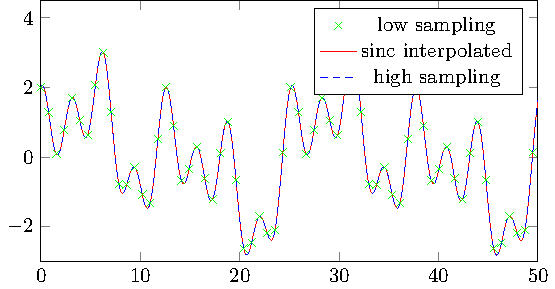
\includegraphics[width=.45\textwidth]{figures/resampling.pdf}
             \caption{The array with low sampling, $\sinc$ interpolation and high sampling all contain the same information.}
             \label{fig:resampling}
         \end{figure}
    

 %   In cases where the input signal is Nyquist sampled, Sinc interpolation can lead
 %   to results which look far superior to classic interpolation schemes
    
 %   \begin{figure}
 %       \centering
 %       \subcaptionbox{$\SI{32}{px}\times\SI{32}{px}$}{\includegraphics[width=.15\textwidth]{%%figures/jinc_small.png}}
   %     \subcaptionbox{\lc{ImageTransformations.imresize}}{
\includegraphics[width=.15\textwid%th]{figures/jinc_imresize.png}}
%        \subcaptionbox{\lc{FourierTools.resample}}{\includegraphics[width=.15\textwidth]{figures/jinc_sinc.png}}
  %      \caption{Caption}
  %      \label{fig:sinc_interp_image}
   % \end{figure}


    \subsection{Subpixel Shifting of Signals}
    
    In \autoref{code:shifting} we show that we can shift a Nyquist sampled signal by an sub pixel amount.
    We evaluate the function \lc{f(x)} shifted by a distance of $0.25$, a quarter of its period. Since the original signal is periodic on the grid and was sampled according to the Nyquist limit, the full information
    of the signal was captured and hence an evaluation of the Fourier series provides identical results up to rounding errors. 
    
    
\begin{lstlisting}[language=Julia, label={code:shifting}, caption={Shifting a Nyquist sampled signal by a sub pixel amount.}, captionpos=b]       
julia> f(x) = sin(x * 2π / 5)
f (generic function with 1 method)

julia> x = 0:4
0:4

julia> transpose(f.(x))
1x5 transpose(::Vector{Float64}) with eltype Float64:
 0.0  0.951057  0.587785  -0.587785  -0.951057

julia> transpose(f.(x .- 0.25))
1x5 transpose(::Vector{Float64}) with eltype Float64:
 -0.309017  0.809017  0.809017  -0.309017  -1.0

julia> transpose(shift(f.(x), 0.25))
1x5 transpose(::Vector{Float64}) with eltype Float64:
 -0.309017  0.809017  0.809017  -0.309017  -1.0
\end{lstlisting}        
Additionally, shifting based on Fourier transforms is also fully revertible, with the only exception being the even--sized Nyquist frequency as mentioned above.

\subsubsection{Handling the Nyquist Amplitude}
In \autoref{code:shifting2} we demonstrate that handling the Nyquist amplitude
in the phase ramp is crucial for correct output results.
Otherwise, shifting a real signal would result in a nonzero imaginary part.
For a real signal one could also take the real part at the end.

\begin{lstlisting}[language=Julia, label={code:shifting2}, caption={Fixing the Nyquist amplitude of the shifting exponential phase ramp.}, captionpos=b] 
julia> x = [1.0, 0.0, 1.0, 0.0];

julia> exp_term = cispi.(2 .* 0.5 .* 
                         fftfreq(size(x, 1))) # shift 0.5 indices
4-element Vector{ComplexF64}:
                1.0 + 0.0im
 0.7071067811865476 + 0.7071067811865476im
                0.0 - 1.0im
 0.7071067811865476 - 0.7071067811865476im
 
julia> ifft(exp_term) # real space kernel is not real
4-element Vector{ComplexF64}:
   0.6035533905932737 - 0.25im
 -0.10355339059327379 + 0.25im
 -0.10355339059327379 - 0.25im
   0.6035533905932737 + 0.25im 
 
julia> ifft(fft(x) .* exp_term) # contains imaginary parts
4-element Vector{ComplexF64}:
 0.5 - 0.5im
 0.5 + 0.5im
 0.5 - 0.5im
 0.5 + 0.5im

julia> exp_term[div(size(x, 1), 2) + 1] = real(exp_term[div(size(x, 1), 2) + 1])
0.0

julia> ifft(exp_term) # real space kernel is real
4-element Vector{ComplexF64}:
   0.6035533905932737 + 0.0im
 -0.10355339059327379 + 0.0im
 -0.10355339059327379 + 0.0im
   0.6035533905932737 + 0.0im


julia> ifft(fft(x) .* exp_term) # real output
4-element Vector{ComplexF64}:
 0.5 + 0.0im
 0.5 + 0.0im
 0.5 + 0.0im
 0.5 + 0.0im
\end{lstlisting}        

Also for complex--valued signals this modification is required, as the real and imaginary part would mix. 
This is demonstrated in \autoref{code:shifting3} where we first shift again
by the na\"ive kernel. And as we can see, shifting the signal with the wrong kernel, can lead to completely wrong results.
% I disagree. I think it is matter of interpretation here.
% There is no right of wrong in this case.
\begin{lstlisting}[language=Julia, label={code:shifting3}, caption={Handling of Nyquist frequency is also for complex signals important.}, captionpos=b] 
julia> x = [1.0 + 1.0im, 0, 1.0 + 1.0im, 0]
4-element Vector{ComplexF64}:
 1.0 + 1.0im
 0.0 + 0.0im
 1.0 + 1.0im
 0.0 + 0.0im

julia> ifft(fft(x) .* cispi.(2 .* 0.5 .*fftfreq(size(x, 1)))) # wrong because of Nyquist amplitude
4-element Vector{ComplexF64}:
 1.0 + 0.0im
 0.0 + 1.0im
 1.0 + 0.0im
 0.0 + 1.0im

julia> shift(x, 0.5) # Using the correct kernel
4-element Vector{ComplexF64}:
 0.5 + 0.5im
 0.5 + 0.5im
 0.5 + 0.5im
 0.5 + 0.5im
\end{lstlisting}        



    \subsection{Shearing and Rotation}
        \autoref{fig:shearandrotation} shows the results of shearing and rotating an image.
        The image is provided by \verb|TestImages.jl|\footnote{\url{https://github.com/JuliaImages/TestImages.jl}}.
        Since we do not resize the image before, the shearing happens completely within the boundaries of the image.
        This circular property is induced by the circularity assumption of the DFT itself.
        The rotated image has even more complex patterns in the boundary regions.
        The reason is that the rotation is based on three shears and hence 
        each shear introduces circular artifacts which are shifted again by following shearing.
        \begin{figure}[h]
            \subcaptionbox{Sheared by \SI{150}{px}.\label{fig:sheared}}{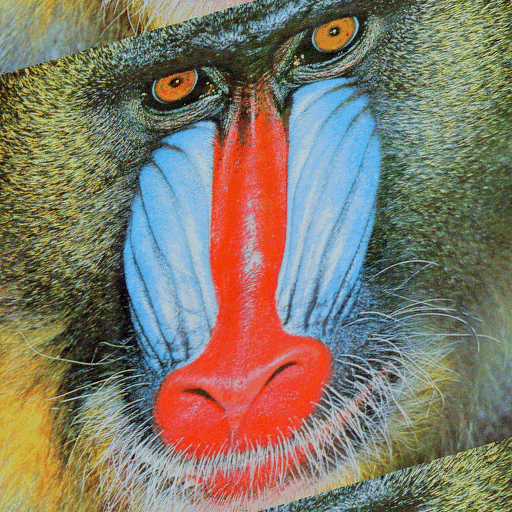
\includegraphics[width=.23\textwidth]{figures/img_sheared.png}}
            \subcaptionbox{Rotated by \SI{50}{\degree}.\label{fig:rotated}}{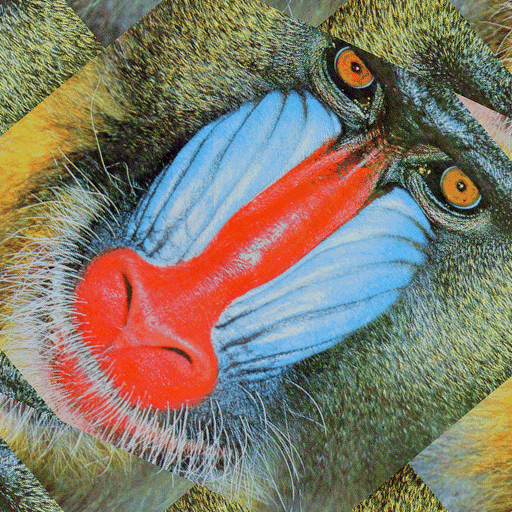
\includegraphics[width=.23\textwidth]{figures/img_rotated.png}}
            \caption{Mandril testimage.}
            \label{fig:shearandrotation}
        \end{figure}
        Fortunately, those artifacts are completely revertible\footnote{in some case the shifting exponential multiplies with $0$ which cannot be recovered.}.
        To rotate without such boundary artifacts, one has to pre-allocate a suitable array beforehand.
        
\section{Conclusion}
    \verb|FourierTools.jl| offers convenient functions to handle data in Fourier space.
    In additon to those functions, we also provide algorithms for different kinds of array manipulation.
    % Hier wird es total Cyptisch!
    The advantage of those algorithms is, that they do not add additional information 
    to the signal but instead rely on the available information
    by reinterpreting the information Fourier space.

\section{Acknowledgement}
We want to thank all people participating in the Discourse discussion\footnote{\url{https://discourse.julialang.org/t/sinc-interpolation-based-on-fft/52512}} and contributing to the clarification of how the boundary is the best handled.
Especially, Steven G. Johnson pointed out the underlying mathematics.


% **************GENERATED FILE, DO NOT EDIT**************

\bibliographystyle{juliacon}
\bibliography{ref.bib}


\end{document}
% Inspired by the International Journal of Computer Applications template
